% Created by tikzDevice version 0.6.2-92-0ad2792 on 2013-03-30 14:52:03
% !TEX encoding = UTF-8 Unicode
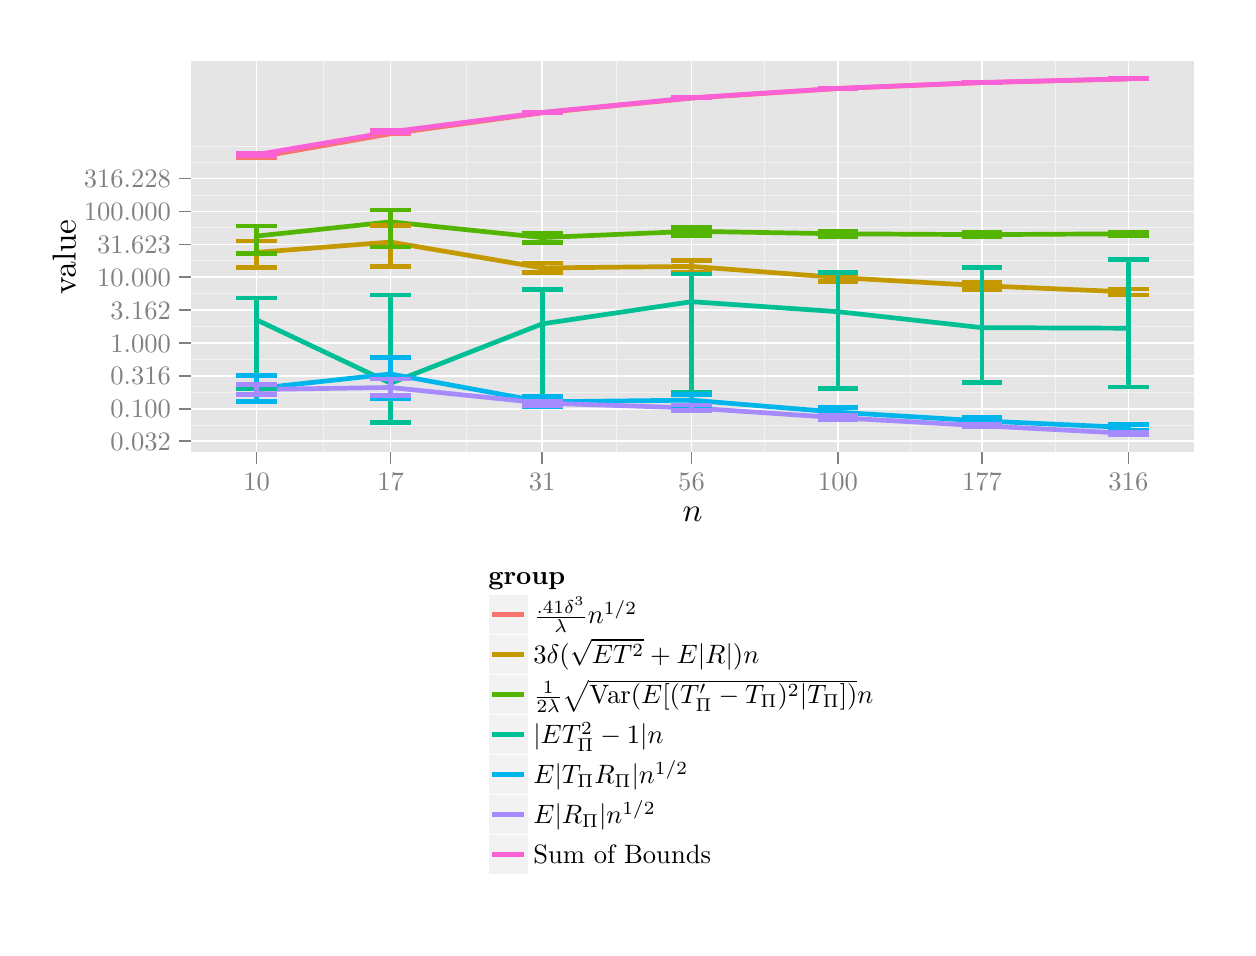
\begin{tikzpicture}[x=1pt,y=1pt]
\definecolor[named]{fillColor}{rgb}{1.00,1.00,1.00}
\path[use as bounding box,fill=fillColor,fill opacity=0.00] (0,0) rectangle (433.62,325.21);
\begin{scope}
\path[clip] (  0.00,  0.00) rectangle (433.62,325.21);
\definecolor[named]{drawColor}{rgb}{1.00,1.00,1.00}
\definecolor[named]{fillColor}{rgb}{1.00,1.00,1.00}

\path[draw=drawColor,line width= 0.6pt,line join=round,line cap=round,fill=fillColor] (  0.00,  0.00) rectangle (433.62,325.21);
\end{scope}
\begin{scope}
\path[clip] ( 58.88,171.72) rectangle (421.57,313.17);
\definecolor[named]{fillColor}{rgb}{0.90,0.90,0.90}

\path[fill=fillColor] ( 58.88,171.72) rectangle (421.57,313.17);
\definecolor[named]{drawColor}{rgb}{0.95,0.95,0.95}

\path[draw=drawColor,line width= 0.3pt,line join=round] ( 58.88,181.65) --
	(421.57,181.65);

\path[draw=drawColor,line width= 0.3pt,line join=round] ( 58.88,193.46) --
	(421.57,193.46);

\path[draw=drawColor,line width= 0.3pt,line join=round] ( 58.88,205.34) --
	(421.57,205.34);

\path[draw=drawColor,line width= 0.3pt,line join=round] ( 58.88,217.22) --
	(421.57,217.22);

\path[draw=drawColor,line width= 0.3pt,line join=round] ( 58.88,229.09) --
	(421.57,229.09);

\path[draw=drawColor,line width= 0.3pt,line join=round] ( 58.88,240.97) --
	(421.57,240.97);

\path[draw=drawColor,line width= 0.3pt,line join=round] ( 58.88,252.85) --
	(421.57,252.85);

\path[draw=drawColor,line width= 0.3pt,line join=round] ( 58.88,264.73) --
	(421.57,264.73);

\path[draw=drawColor,line width= 0.3pt,line join=round] ( 58.88,276.54) --
	(421.57,276.54);

\path[draw=drawColor,line width= 0.3pt,line join=round] ( 58.88,282.42) --
	(421.57,282.42);

\path[draw=drawColor,line width= 0.3pt,line join=round] (106.92,171.72) --
	(106.92,313.17);

\path[draw=drawColor,line width= 0.3pt,line join=round] (158.53,171.72) --
	(158.53,313.17);

\path[draw=drawColor,line width= 0.3pt,line join=round] (212.91,171.72) --
	(212.91,313.17);

\path[draw=drawColor,line width= 0.3pt,line join=round] (266.33,171.72) --
	(266.33,313.17);

\path[draw=drawColor,line width= 0.3pt,line join=round] (318.82,171.72) --
	(318.82,313.17);

\path[draw=drawColor,line width= 0.3pt,line join=round] (371.30,171.72) --
	(371.30,313.17);
\definecolor[named]{drawColor}{rgb}{1.00,1.00,1.00}

\path[draw=drawColor,line width= 0.6pt,line join=round] ( 58.88,175.77) --
	(421.57,175.77);

\path[draw=drawColor,line width= 0.6pt,line join=round] ( 58.88,187.53) --
	(421.57,187.53);

\path[draw=drawColor,line width= 0.6pt,line join=round] ( 58.88,199.40) --
	(421.57,199.40);

\path[draw=drawColor,line width= 0.6pt,line join=round] ( 58.88,211.28) --
	(421.57,211.28);

\path[draw=drawColor,line width= 0.6pt,line join=round] ( 58.88,223.16) --
	(421.57,223.16);

\path[draw=drawColor,line width= 0.6pt,line join=round] ( 58.88,235.03) --
	(421.57,235.03);

\path[draw=drawColor,line width= 0.6pt,line join=round] ( 58.88,246.91) --
	(421.57,246.91);

\path[draw=drawColor,line width= 0.6pt,line join=round] ( 58.88,258.79) --
	(421.57,258.79);

\path[draw=drawColor,line width= 0.6pt,line join=round] ( 58.88,270.66) --
	(421.57,270.66);

\path[draw=drawColor,line width= 0.6pt,line join=round] ( 82.72,171.72) --
	( 82.72,313.17);

\path[draw=drawColor,line width= 0.6pt,line join=round] (131.13,171.72) --
	(131.13,313.17);

\path[draw=drawColor,line width= 0.6pt,line join=round] (185.93,171.72) --
	(185.93,313.17);

\path[draw=drawColor,line width= 0.6pt,line join=round] (239.88,171.72) --
	(239.88,313.17);

\path[draw=drawColor,line width= 0.6pt,line join=round] (292.78,171.72) --
	(292.78,313.17);

\path[draw=drawColor,line width= 0.6pt,line join=round] (344.86,171.72) --
	(344.86,313.17);

\path[draw=drawColor,line width= 0.6pt,line join=round] (397.74,171.72) --
	(397.74,313.17);
\definecolor[named]{drawColor}{rgb}{0.97,0.46,0.43}

\path[draw=drawColor,line width= 1.7pt,line join=round] ( 82.72,278.33) --
	(131.13,286.86) --
	(185.93,294.43) --
	(239.88,299.74) --
	(292.78,303.20) --
	(344.86,305.35) --
	(397.74,306.67);
\definecolor[named]{drawColor}{rgb}{0.77,0.60,0.00}

\path[draw=drawColor,line width= 1.7pt,line join=round] ( 82.72,244.00) --
	(131.13,247.73) --
	(185.93,238.39) --
	(239.88,238.94) --
	(292.78,234.92) --
	(344.86,231.97) --
	(397.74,229.70);
\definecolor[named]{drawColor}{rgb}{0.33,0.71,0.00}

\path[draw=drawColor,line width= 1.7pt,line join=round] ( 82.72,249.90) --
	(131.13,255.04) --
	(185.93,249.36) --
	(239.88,251.63) --
	(292.78,250.73) --
	(344.86,250.42) --
	(397.74,250.73);
\definecolor[named]{drawColor}{rgb}{0.00,0.75,0.58}

\path[draw=drawColor,line width= 1.7pt,line join=round] ( 82.72,219.63) --
	(131.13,196.73) --
	(185.93,218.18) --
	(239.88,226.19) --
	(292.78,222.58) --
	(344.86,216.81) --
	(397.74,216.61);
\definecolor[named]{drawColor}{rgb}{0.00,0.71,0.92}

\path[draw=drawColor,line width= 1.7pt,line join=round] ( 82.72,194.83) --
	(131.13,200.06) --
	(185.93,190.02) --
	(239.88,190.61) --
	(292.78,186.24) --
	(344.86,183.11) --
	(397.74,180.72);
\definecolor[named]{drawColor}{rgb}{0.65,0.54,1.00}

\path[draw=drawColor,line width= 1.7pt,line join=round] ( 82.72,194.46) --
	(131.13,195.19) --
	(185.93,189.55) --
	(239.88,187.81) --
	(292.78,184.27) --
	(344.86,181.36) --
	(397.74,178.60);
\definecolor[named]{drawColor}{rgb}{0.98,0.38,0.84}

\path[draw=drawColor,line width= 1.7pt,line join=round] ( 82.72,279.34) --
	(131.13,287.55) --
	(185.93,294.61) --
	(239.88,299.87) --
	(292.78,303.28) --
	(344.86,305.41) --
	(397.74,306.73);
\definecolor[named]{drawColor}{rgb}{0.97,0.46,0.43}

\path[draw=drawColor,line width= 1.7pt,line join=round] ( 75.37,278.33) --
	( 90.07,278.33);

\path[draw=drawColor,line width= 1.7pt,line join=round] ( 82.72,278.33) --
	( 82.72,278.33);

\path[draw=drawColor,line width= 1.7pt,line join=round] ( 75.37,278.33) --
	( 90.07,278.33);

\path[draw=drawColor,line width= 1.7pt,line join=round] (123.78,286.86) --
	(138.48,286.86);

\path[draw=drawColor,line width= 1.7pt,line join=round] (131.13,286.86) --
	(131.13,286.86);

\path[draw=drawColor,line width= 1.7pt,line join=round] (123.78,286.86) --
	(138.48,286.86);

\path[draw=drawColor,line width= 1.7pt,line join=round] (178.58,294.43) --
	(193.28,294.43);

\path[draw=drawColor,line width= 1.7pt,line join=round] (185.93,294.43) --
	(185.93,294.43);

\path[draw=drawColor,line width= 1.7pt,line join=round] (178.58,294.43) --
	(193.28,294.43);

\path[draw=drawColor,line width= 1.7pt,line join=round] (232.53,299.74) --
	(247.23,299.74);

\path[draw=drawColor,line width= 1.7pt,line join=round] (239.88,299.74) --
	(239.88,299.74);

\path[draw=drawColor,line width= 1.7pt,line join=round] (232.53,299.74) --
	(247.23,299.74);

\path[draw=drawColor,line width= 1.7pt,line join=round] (285.42,303.20) --
	(300.13,303.20);

\path[draw=drawColor,line width= 1.7pt,line join=round] (292.78,303.20) --
	(292.78,303.20);

\path[draw=drawColor,line width= 1.7pt,line join=round] (285.42,303.20) --
	(300.13,303.20);

\path[draw=drawColor,line width= 1.7pt,line join=round] (337.51,305.35) --
	(352.22,305.35);

\path[draw=drawColor,line width= 1.7pt,line join=round] (344.86,305.35) --
	(344.86,305.35);

\path[draw=drawColor,line width= 1.7pt,line join=round] (337.51,305.35) --
	(352.22,305.35);

\path[draw=drawColor,line width= 1.7pt,line join=round] (390.39,306.67) --
	(405.09,306.67);

\path[draw=drawColor,line width= 1.7pt,line join=round] (397.74,306.67) --
	(397.74,306.67);

\path[draw=drawColor,line width= 1.7pt,line join=round] (390.39,306.67) --
	(405.09,306.67);
\definecolor[named]{drawColor}{rgb}{0.77,0.60,0.00}

\path[draw=drawColor,line width= 1.7pt,line join=round] ( 75.37,248.11) --
	( 90.07,248.11);

\path[draw=drawColor,line width= 1.7pt,line join=round] ( 82.72,248.11) --
	( 82.72,238.51);

\path[draw=drawColor,line width= 1.7pt,line join=round] ( 75.37,238.51) --
	( 90.07,238.51);

\path[draw=drawColor,line width= 1.7pt,line join=round] (123.78,253.63) --
	(138.48,253.63);

\path[draw=drawColor,line width= 1.7pt,line join=round] (131.13,253.63) --
	(131.13,238.85);

\path[draw=drawColor,line width= 1.7pt,line join=round] (123.78,238.85) --
	(138.48,238.85);

\path[draw=drawColor,line width= 1.7pt,line join=round] (178.58,240.12) --
	(193.28,240.12);

\path[draw=drawColor,line width= 1.7pt,line join=round] (185.93,240.12) --
	(185.93,236.64);

\path[draw=drawColor,line width= 1.7pt,line join=round] (178.58,236.64) --
	(193.28,236.64);

\path[draw=drawColor,line width= 1.7pt,line join=round] (232.53,241.15) --
	(247.23,241.15);

\path[draw=drawColor,line width= 1.7pt,line join=round] (239.88,241.15) --
	(239.88,236.68);

\path[draw=drawColor,line width= 1.7pt,line join=round] (232.53,236.68) --
	(247.23,236.68);

\path[draw=drawColor,line width= 1.7pt,line join=round] (285.42,236.37) --
	(300.13,236.37);

\path[draw=drawColor,line width= 1.7pt,line join=round] (292.78,236.37) --
	(292.78,233.40);

\path[draw=drawColor,line width= 1.7pt,line join=round] (285.42,233.40) --
	(300.13,233.40);

\path[draw=drawColor,line width= 1.7pt,line join=round] (337.51,233.18) --
	(352.22,233.18);

\path[draw=drawColor,line width= 1.7pt,line join=round] (344.86,233.18) --
	(344.86,230.66);

\path[draw=drawColor,line width= 1.7pt,line join=round] (337.51,230.66) --
	(352.22,230.66);

\path[draw=drawColor,line width= 1.7pt,line join=round] (390.39,230.81) --
	(405.09,230.81);

\path[draw=drawColor,line width= 1.7pt,line join=round] (397.74,230.81) --
	(397.74,228.62);

\path[draw=drawColor,line width= 1.7pt,line join=round] (390.39,228.62) --
	(405.09,228.62);
\definecolor[named]{drawColor}{rgb}{0.33,0.71,0.00}

\path[draw=drawColor,line width= 1.7pt,line join=round] ( 75.37,253.54) --
	( 90.07,253.54);

\path[draw=drawColor,line width= 1.7pt,line join=round] ( 82.72,253.54) --
	( 82.72,243.64);

\path[draw=drawColor,line width= 1.7pt,line join=round] ( 75.37,243.64) --
	( 90.07,243.64);

\path[draw=drawColor,line width= 1.7pt,line join=round] (123.78,259.31) --
	(138.48,259.31);

\path[draw=drawColor,line width= 1.7pt,line join=round] (131.13,259.31) --
	(131.13,245.96);

\path[draw=drawColor,line width= 1.7pt,line join=round] (123.78,245.96) --
	(138.48,245.96);

\path[draw=drawColor,line width= 1.7pt,line join=round] (178.58,250.87) --
	(193.28,250.87);

\path[draw=drawColor,line width= 1.7pt,line join=round] (185.93,250.87) --
	(185.93,247.60);

\path[draw=drawColor,line width= 1.7pt,line join=round] (178.58,247.60) --
	(193.28,247.60);

\path[draw=drawColor,line width= 1.7pt,line join=round] (232.53,252.90) --
	(247.23,252.90);

\path[draw=drawColor,line width= 1.7pt,line join=round] (239.88,252.90) --
	(239.88,250.11);

\path[draw=drawColor,line width= 1.7pt,line join=round] (232.53,250.11) --
	(247.23,250.11);

\path[draw=drawColor,line width= 1.7pt,line join=round] (285.42,251.68) --
	(300.13,251.68);

\path[draw=drawColor,line width= 1.7pt,line join=round] (292.78,251.68) --
	(292.78,249.67);

\path[draw=drawColor,line width= 1.7pt,line join=round] (285.42,249.67) --
	(300.13,249.67);

\path[draw=drawColor,line width= 1.7pt,line join=round] (337.51,251.19) --
	(352.22,251.19);

\path[draw=drawColor,line width= 1.7pt,line join=round] (344.86,251.19) --
	(344.86,249.58);

\path[draw=drawColor,line width= 1.7pt,line join=round] (337.51,249.58) --
	(352.22,249.58);

\path[draw=drawColor,line width= 1.7pt,line join=round] (390.39,251.34) --
	(405.09,251.34);

\path[draw=drawColor,line width= 1.7pt,line join=round] (397.74,251.34) --
	(397.74,250.08);

\path[draw=drawColor,line width= 1.7pt,line join=round] (390.39,250.08) --
	(405.09,250.08);
\definecolor[named]{drawColor}{rgb}{0.00,0.75,0.58}

\path[draw=drawColor,line width= 1.7pt,line join=round] ( 75.37,227.55) --
	( 90.07,227.55);

\path[draw=drawColor,line width= 1.7pt,line join=round] ( 82.72,227.55) --
	( 82.72,194.72);

\path[draw=drawColor,line width= 1.7pt,line join=round] ( 75.37,194.72) --
	( 90.07,194.72);

\path[draw=drawColor,line width= 1.7pt,line join=round] (123.78,228.63) --
	(138.48,228.63);

\path[draw=drawColor,line width= 1.7pt,line join=round] (131.13,228.63) --
	(131.13,182.45);

\path[draw=drawColor,line width= 1.7pt,line join=round] (123.78,182.45) --
	(138.48,182.45);

\path[draw=drawColor,line width= 1.7pt,line join=round] (178.58,230.66) --
	(193.28,230.66);

\path[draw=drawColor,line width= 1.7pt,line join=round] (185.93,230.66) --
	(185.93,188.75);

\path[draw=drawColor,line width= 1.7pt,line join=round] (178.58,188.75) --
	(193.28,188.75);

\path[draw=drawColor,line width= 1.7pt,line join=round] (232.53,236.16) --
	(247.23,236.16);

\path[draw=drawColor,line width= 1.7pt,line join=round] (239.88,236.16) --
	(239.88,193.36);

\path[draw=drawColor,line width= 1.7pt,line join=round] (232.53,193.36) --
	(247.23,193.36);

\path[draw=drawColor,line width= 1.7pt,line join=round] (285.42,236.63) --
	(300.13,236.63);

\path[draw=drawColor,line width= 1.7pt,line join=round] (292.78,236.63) --
	(292.78,194.79);

\path[draw=drawColor,line width= 1.7pt,line join=round] (285.42,194.79) --
	(300.13,194.79);

\path[draw=drawColor,line width= 1.7pt,line join=round] (337.51,238.64) --
	(352.22,238.64);

\path[draw=drawColor,line width= 1.7pt,line join=round] (344.86,238.64) --
	(344.86,196.95);

\path[draw=drawColor,line width= 1.7pt,line join=round] (337.51,196.95) --
	(352.22,196.95);

\path[draw=drawColor,line width= 1.7pt,line join=round] (390.39,241.34) --
	(405.09,241.34);

\path[draw=drawColor,line width= 1.7pt,line join=round] (397.74,241.34) --
	(397.74,195.37);

\path[draw=drawColor,line width= 1.7pt,line join=round] (390.39,195.37) --
	(405.09,195.37);
\definecolor[named]{drawColor}{rgb}{0.00,0.71,0.92}

\path[draw=drawColor,line width= 1.7pt,line join=round] ( 75.37,199.45) --
	( 90.07,199.45);

\path[draw=drawColor,line width= 1.7pt,line join=round] ( 82.72,199.45) --
	( 82.72,190.12);

\path[draw=drawColor,line width= 1.7pt,line join=round] ( 75.37,190.12) --
	( 90.07,190.12);

\path[draw=drawColor,line width= 1.7pt,line join=round] (123.78,205.94) --
	(138.48,205.94);

\path[draw=drawColor,line width= 1.7pt,line join=round] (131.13,205.94) --
	(131.13,191.11);

\path[draw=drawColor,line width= 1.7pt,line join=round] (123.78,191.11) --
	(138.48,191.11);

\path[draw=drawColor,line width= 1.7pt,line join=round] (178.58,191.84) --
	(193.28,191.84);

\path[draw=drawColor,line width= 1.7pt,line join=round] (185.93,191.84) --
	(185.93,188.15);

\path[draw=drawColor,line width= 1.7pt,line join=round] (178.58,188.15) --
	(193.28,188.15);

\path[draw=drawColor,line width= 1.7pt,line join=round] (232.53,192.71) --
	(247.23,192.71);

\path[draw=drawColor,line width= 1.7pt,line join=round] (239.88,192.71) --
	(239.88,188.05);

\path[draw=drawColor,line width= 1.7pt,line join=round] (232.53,188.05) --
	(247.23,188.05);

\path[draw=drawColor,line width= 1.7pt,line join=round] (285.42,187.91) --
	(300.13,187.91);

\path[draw=drawColor,line width= 1.7pt,line join=round] (292.78,187.91) --
	(292.78,184.55);

\path[draw=drawColor,line width= 1.7pt,line join=round] (285.42,184.55) --
	(300.13,184.55);

\path[draw=drawColor,line width= 1.7pt,line join=round] (337.51,184.41) --
	(352.22,184.41);

\path[draw=drawColor,line width= 1.7pt,line join=round] (344.86,184.41) --
	(344.86,181.78);

\path[draw=drawColor,line width= 1.7pt,line join=round] (337.51,181.78) --
	(352.22,181.78);

\path[draw=drawColor,line width= 1.7pt,line join=round] (390.39,181.76) --
	(405.09,181.76);

\path[draw=drawColor,line width= 1.7pt,line join=round] (397.74,181.76) --
	(397.74,179.53);

\path[draw=drawColor,line width= 1.7pt,line join=round] (390.39,179.53) --
	(405.09,179.53);
\definecolor[named]{drawColor}{rgb}{0.65,0.54,1.00}

\path[draw=drawColor,line width= 1.7pt,line join=round] ( 75.37,196.38) --
	( 90.07,196.38);

\path[draw=drawColor,line width= 1.7pt,line join=round] ( 82.72,196.38) --
	( 82.72,192.76);

\path[draw=drawColor,line width= 1.7pt,line join=round] ( 75.37,192.76) --
	( 90.07,192.76);

\path[draw=drawColor,line width= 1.7pt,line join=round] (123.78,198.24) --
	(138.48,198.24);

\path[draw=drawColor,line width= 1.7pt,line join=round] (131.13,198.24) --
	(131.13,192.32);

\path[draw=drawColor,line width= 1.7pt,line join=round] (123.78,192.32) --
	(138.48,192.32);

\path[draw=drawColor,line width= 1.7pt,line join=round] (178.58,190.33) --
	(193.28,190.33);

\path[draw=drawColor,line width= 1.7pt,line join=round] (185.93,190.33) --
	(185.93,188.75);

\path[draw=drawColor,line width= 1.7pt,line join=round] (178.58,188.75) --
	(193.28,188.75);

\path[draw=drawColor,line width= 1.7pt,line join=round] (232.53,188.88) --
	(247.23,188.88);

\path[draw=drawColor,line width= 1.7pt,line join=round] (239.88,188.88) --
	(239.88,186.80);

\path[draw=drawColor,line width= 1.7pt,line join=round] (232.53,186.80) --
	(247.23,186.80);

\path[draw=drawColor,line width= 1.7pt,line join=round] (285.42,184.98) --
	(300.13,184.98);

\path[draw=drawColor,line width= 1.7pt,line join=round] (292.78,184.98) --
	(292.78,183.58);

\path[draw=drawColor,line width= 1.7pt,line join=round] (285.42,183.58) --
	(300.13,183.58);

\path[draw=drawColor,line width= 1.7pt,line join=round] (337.51,181.92) --
	(352.22,181.92);

\path[draw=drawColor,line width= 1.7pt,line join=round] (344.86,181.92) --
	(344.86,180.86);

\path[draw=drawColor,line width= 1.7pt,line join=round] (337.51,180.86) --
	(352.22,180.86);

\path[draw=drawColor,line width= 1.7pt,line join=round] (390.39,179.03) --
	(405.09,179.03);

\path[draw=drawColor,line width= 1.7pt,line join=round] (397.74,179.03) --
	(397.74,178.15);

\path[draw=drawColor,line width= 1.7pt,line join=round] (390.39,178.15) --
	(405.09,178.15);
\definecolor[named]{drawColor}{rgb}{0.98,0.38,0.84}

\path[draw=drawColor,line width= 1.7pt,line join=round] ( 75.37,279.70) --
	( 90.07,279.70);

\path[draw=drawColor,line width= 1.7pt,line join=round] ( 82.72,279.70) --
	( 82.72,278.96);

\path[draw=drawColor,line width= 1.7pt,line join=round] ( 75.37,278.96) --
	( 90.07,278.96);

\path[draw=drawColor,line width= 1.7pt,line join=round] (123.78,287.94) --
	(138.48,287.94);

\path[draw=drawColor,line width= 1.7pt,line join=round] (131.13,287.94) --
	(131.13,287.17);

\path[draw=drawColor,line width= 1.7pt,line join=round] (123.78,287.17) --
	(138.48,287.17);

\path[draw=drawColor,line width= 1.7pt,line join=round] (178.58,294.63) --
	(193.28,294.63);

\path[draw=drawColor,line width= 1.7pt,line join=round] (185.93,294.63) --
	(185.93,294.59);

\path[draw=drawColor,line width= 1.7pt,line join=round] (178.58,294.59) --
	(193.28,294.59);

\path[draw=drawColor,line width= 1.7pt,line join=round] (232.53,299.90) --
	(247.23,299.90);

\path[draw=drawColor,line width= 1.7pt,line join=round] (239.88,299.90) --
	(239.88,299.85);

\path[draw=drawColor,line width= 1.7pt,line join=round] (232.53,299.85) --
	(247.23,299.85);

\path[draw=drawColor,line width= 1.7pt,line join=round] (285.42,303.30) --
	(300.13,303.30);

\path[draw=drawColor,line width= 1.7pt,line join=round] (292.78,303.30) --
	(292.78,303.27);

\path[draw=drawColor,line width= 1.7pt,line join=round] (285.42,303.27) --
	(300.13,303.27);

\path[draw=drawColor,line width= 1.7pt,line join=round] (337.51,305.43) --
	(352.22,305.43);

\path[draw=drawColor,line width= 1.7pt,line join=round] (344.86,305.43) --
	(344.86,305.41);

\path[draw=drawColor,line width= 1.7pt,line join=round] (337.51,305.41) --
	(352.22,305.41);

\path[draw=drawColor,line width= 1.7pt,line join=round] (390.39,306.74) --
	(405.09,306.74);

\path[draw=drawColor,line width= 1.7pt,line join=round] (397.74,306.74) --
	(397.74,306.72);

\path[draw=drawColor,line width= 1.7pt,line join=round] (390.39,306.72) --
	(405.09,306.72);
\end{scope}
\begin{scope}
\path[clip] (  0.00,  0.00) rectangle (433.62,325.21);
\definecolor[named]{drawColor}{rgb}{0.50,0.50,0.50}

\node[text=drawColor,anchor=base east,inner sep=0pt, outer sep=0pt, scale=  0.96] at ( 51.77,172.47) {0.032};

\node[text=drawColor,anchor=base east,inner sep=0pt, outer sep=0pt, scale=  0.96] at ( 51.77,184.22) {0.100};

\node[text=drawColor,anchor=base east,inner sep=0pt, outer sep=0pt, scale=  0.96] at ( 51.77,196.09) {0.316};

\node[text=drawColor,anchor=base east,inner sep=0pt, outer sep=0pt, scale=  0.96] at ( 51.77,207.97) {1.000};

\node[text=drawColor,anchor=base east,inner sep=0pt, outer sep=0pt, scale=  0.96] at ( 51.77,219.85) {3.162};

\node[text=drawColor,anchor=base east,inner sep=0pt, outer sep=0pt, scale=  0.96] at ( 51.77,231.73) {10.000};

\node[text=drawColor,anchor=base east,inner sep=0pt, outer sep=0pt, scale=  0.96] at ( 51.77,243.60) {31.623};

\node[text=drawColor,anchor=base east,inner sep=0pt, outer sep=0pt, scale=  0.96] at ( 51.77,255.48) {100.000};

\node[text=drawColor,anchor=base east,inner sep=0pt, outer sep=0pt, scale=  0.96] at ( 51.77,267.36) {316.228};
\end{scope}
\begin{scope}
\path[clip] (  0.00,  0.00) rectangle (433.62,325.21);
\definecolor[named]{drawColor}{rgb}{0.50,0.50,0.50}

\path[draw=drawColor,line width= 0.6pt,line join=round] ( 54.61,175.77) --
	( 58.88,175.77);

\path[draw=drawColor,line width= 0.6pt,line join=round] ( 54.61,187.53) --
	( 58.88,187.53);

\path[draw=drawColor,line width= 0.6pt,line join=round] ( 54.61,199.40) --
	( 58.88,199.40);

\path[draw=drawColor,line width= 0.6pt,line join=round] ( 54.61,211.28) --
	( 58.88,211.28);

\path[draw=drawColor,line width= 0.6pt,line join=round] ( 54.61,223.16) --
	( 58.88,223.16);

\path[draw=drawColor,line width= 0.6pt,line join=round] ( 54.61,235.03) --
	( 58.88,235.03);

\path[draw=drawColor,line width= 0.6pt,line join=round] ( 54.61,246.91) --
	( 58.88,246.91);

\path[draw=drawColor,line width= 0.6pt,line join=round] ( 54.61,258.79) --
	( 58.88,258.79);

\path[draw=drawColor,line width= 0.6pt,line join=round] ( 54.61,270.66) --
	( 58.88,270.66);
\end{scope}
\begin{scope}
\path[clip] (  0.00,  0.00) rectangle (433.62,325.21);
\definecolor[named]{drawColor}{rgb}{0.50,0.50,0.50}

\path[draw=drawColor,line width= 0.6pt,line join=round] ( 82.72,167.45) --
	( 82.72,171.72);

\path[draw=drawColor,line width= 0.6pt,line join=round] (131.13,167.45) --
	(131.13,171.72);

\path[draw=drawColor,line width= 0.6pt,line join=round] (185.93,167.45) --
	(185.93,171.72);

\path[draw=drawColor,line width= 0.6pt,line join=round] (239.88,167.45) --
	(239.88,171.72);

\path[draw=drawColor,line width= 0.6pt,line join=round] (292.78,167.45) --
	(292.78,171.72);

\path[draw=drawColor,line width= 0.6pt,line join=round] (344.86,167.45) --
	(344.86,171.72);

\path[draw=drawColor,line width= 0.6pt,line join=round] (397.74,167.45) --
	(397.74,171.72);
\end{scope}
\begin{scope}
\path[clip] (  0.00,  0.00) rectangle (433.62,325.21);
\definecolor[named]{drawColor}{rgb}{0.50,0.50,0.50}

\node[text=drawColor,anchor=base,inner sep=0pt, outer sep=0pt, scale=  0.96] at ( 82.72,158.00) {10};

\node[text=drawColor,anchor=base,inner sep=0pt, outer sep=0pt, scale=  0.96] at (131.13,158.00) {17};

\node[text=drawColor,anchor=base,inner sep=0pt, outer sep=0pt, scale=  0.96] at (185.93,158.00) {31};

\node[text=drawColor,anchor=base,inner sep=0pt, outer sep=0pt, scale=  0.96] at (239.88,158.00) {56};

\node[text=drawColor,anchor=base,inner sep=0pt, outer sep=0pt, scale=  0.96] at (292.78,158.00) {100};

\node[text=drawColor,anchor=base,inner sep=0pt, outer sep=0pt, scale=  0.96] at (344.86,158.00) {177};

\node[text=drawColor,anchor=base,inner sep=0pt, outer sep=0pt, scale=  0.96] at (397.74,158.00) {316};
\end{scope}
\begin{scope}
\path[clip] (  0.00,  0.00) rectangle (433.62,325.21);
\definecolor[named]{drawColor}{rgb}{0.00,0.00,0.00}

\node[text=drawColor,anchor=base,inner sep=0pt, outer sep=0pt, scale=  1.20] at (240.23,146.72) {$n$};
\end{scope}
\begin{scope}
\path[clip] (  0.00,  0.00) rectangle (433.62,325.21);
\definecolor[named]{drawColor}{rgb}{0.00,0.00,0.00}

\node[text=drawColor,rotate= 90.00,anchor=base,inner sep=0pt, outer sep=0pt, scale=  1.20] at ( 17.30,242.45) {value};
\end{scope}
\begin{scope}
\path[clip] (  0.00,  0.00) rectangle (433.62,325.21);
\definecolor[named]{fillColor}{rgb}{1.00,1.00,1.00}

\path[fill=fillColor] (162.21, 14.89) rectangle (318.25,134.84);
\end{scope}
\begin{scope}
\path[clip] (  0.00,  0.00) rectangle (433.62,325.21);
\definecolor[named]{drawColor}{rgb}{0.00,0.00,0.00}

\node[text=drawColor,anchor=base west,inner sep=0pt, outer sep=0pt, scale=  0.96] at (166.47,123.95) {\bfseries group};
\end{scope}
\begin{scope}
\path[clip] (  0.00,  0.00) rectangle (433.62,325.21);
\definecolor[named]{drawColor}{rgb}{1.00,1.00,1.00}
\definecolor[named]{fillColor}{rgb}{0.95,0.95,0.95}

\path[draw=drawColor,line width= 0.6pt,line join=round,line cap=round,fill=fillColor] (166.47,105.88) rectangle (180.93,120.34);
\end{scope}
\begin{scope}
\path[clip] (  0.00,  0.00) rectangle (433.62,325.21);
\definecolor[named]{drawColor}{rgb}{0.97,0.46,0.43}

\path[draw=drawColor,line width= 1.7pt,line join=round] (167.92,113.11) -- (179.48,113.11);
\end{scope}
\begin{scope}
\path[clip] (  0.00,  0.00) rectangle (433.62,325.21);
\definecolor[named]{drawColor}{rgb}{0.97,0.46,0.43}

\path[draw=drawColor,line width= 1.7pt,line join=round] (167.92,113.11) -- (179.48,113.11);
\end{scope}
\begin{scope}
\path[clip] (  0.00,  0.00) rectangle (433.62,325.21);
\definecolor[named]{drawColor}{rgb}{1.00,1.00,1.00}
\definecolor[named]{fillColor}{rgb}{0.95,0.95,0.95}

\path[draw=drawColor,line width= 0.6pt,line join=round,line cap=round,fill=fillColor] (166.47, 91.43) rectangle (180.93,105.88);
\end{scope}
\begin{scope}
\path[clip] (  0.00,  0.00) rectangle (433.62,325.21);
\definecolor[named]{drawColor}{rgb}{0.77,0.60,0.00}

\path[draw=drawColor,line width= 1.7pt,line join=round] (167.92, 98.66) -- (179.48, 98.66);
\end{scope}
\begin{scope}
\path[clip] (  0.00,  0.00) rectangle (433.62,325.21);
\definecolor[named]{drawColor}{rgb}{0.77,0.60,0.00}

\path[draw=drawColor,line width= 1.7pt,line join=round] (167.92, 98.66) -- (179.48, 98.66);
\end{scope}
\begin{scope}
\path[clip] (  0.00,  0.00) rectangle (433.62,325.21);
\definecolor[named]{drawColor}{rgb}{1.00,1.00,1.00}
\definecolor[named]{fillColor}{rgb}{0.95,0.95,0.95}

\path[draw=drawColor,line width= 0.6pt,line join=round,line cap=round,fill=fillColor] (166.47, 76.97) rectangle (180.93, 91.43);
\end{scope}
\begin{scope}
\path[clip] (  0.00,  0.00) rectangle (433.62,325.21);
\definecolor[named]{drawColor}{rgb}{0.33,0.71,0.00}

\path[draw=drawColor,line width= 1.7pt,line join=round] (167.92, 84.20) -- (179.48, 84.20);
\end{scope}
\begin{scope}
\path[clip] (  0.00,  0.00) rectangle (433.62,325.21);
\definecolor[named]{drawColor}{rgb}{0.33,0.71,0.00}

\path[draw=drawColor,line width= 1.7pt,line join=round] (167.92, 84.20) -- (179.48, 84.20);
\end{scope}
\begin{scope}
\path[clip] (  0.00,  0.00) rectangle (433.62,325.21);
\definecolor[named]{drawColor}{rgb}{1.00,1.00,1.00}
\definecolor[named]{fillColor}{rgb}{0.95,0.95,0.95}

\path[draw=drawColor,line width= 0.6pt,line join=round,line cap=round,fill=fillColor] (166.47, 62.52) rectangle (180.93, 76.97);
\end{scope}
\begin{scope}
\path[clip] (  0.00,  0.00) rectangle (433.62,325.21);
\definecolor[named]{drawColor}{rgb}{0.00,0.75,0.58}

\path[draw=drawColor,line width= 1.7pt,line join=round] (167.92, 69.75) -- (179.48, 69.75);
\end{scope}
\begin{scope}
\path[clip] (  0.00,  0.00) rectangle (433.62,325.21);
\definecolor[named]{drawColor}{rgb}{0.00,0.75,0.58}

\path[draw=drawColor,line width= 1.7pt,line join=round] (167.92, 69.75) -- (179.48, 69.75);
\end{scope}
\begin{scope}
\path[clip] (  0.00,  0.00) rectangle (433.62,325.21);
\definecolor[named]{drawColor}{rgb}{1.00,1.00,1.00}
\definecolor[named]{fillColor}{rgb}{0.95,0.95,0.95}

\path[draw=drawColor,line width= 0.6pt,line join=round,line cap=round,fill=fillColor] (166.47, 48.07) rectangle (180.93, 62.52);
\end{scope}
\begin{scope}
\path[clip] (  0.00,  0.00) rectangle (433.62,325.21);
\definecolor[named]{drawColor}{rgb}{0.00,0.71,0.92}

\path[draw=drawColor,line width= 1.7pt,line join=round] (167.92, 55.29) -- (179.48, 55.29);
\end{scope}
\begin{scope}
\path[clip] (  0.00,  0.00) rectangle (433.62,325.21);
\definecolor[named]{drawColor}{rgb}{0.00,0.71,0.92}

\path[draw=drawColor,line width= 1.7pt,line join=round] (167.92, 55.29) -- (179.48, 55.29);
\end{scope}
\begin{scope}
\path[clip] (  0.00,  0.00) rectangle (433.62,325.21);
\definecolor[named]{drawColor}{rgb}{1.00,1.00,1.00}
\definecolor[named]{fillColor}{rgb}{0.95,0.95,0.95}

\path[draw=drawColor,line width= 0.6pt,line join=round,line cap=round,fill=fillColor] (166.47, 33.61) rectangle (180.93, 48.07);
\end{scope}
\begin{scope}
\path[clip] (  0.00,  0.00) rectangle (433.62,325.21);
\definecolor[named]{drawColor}{rgb}{0.65,0.54,1.00}

\path[draw=drawColor,line width= 1.7pt,line join=round] (167.92, 40.84) -- (179.48, 40.84);
\end{scope}
\begin{scope}
\path[clip] (  0.00,  0.00) rectangle (433.62,325.21);
\definecolor[named]{drawColor}{rgb}{0.65,0.54,1.00}

\path[draw=drawColor,line width= 1.7pt,line join=round] (167.92, 40.84) -- (179.48, 40.84);
\end{scope}
\begin{scope}
\path[clip] (  0.00,  0.00) rectangle (433.62,325.21);
\definecolor[named]{drawColor}{rgb}{1.00,1.00,1.00}
\definecolor[named]{fillColor}{rgb}{0.95,0.95,0.95}

\path[draw=drawColor,line width= 0.6pt,line join=round,line cap=round,fill=fillColor] (166.47, 19.16) rectangle (180.93, 33.61);
\end{scope}
\begin{scope}
\path[clip] (  0.00,  0.00) rectangle (433.62,325.21);
\definecolor[named]{drawColor}{rgb}{0.98,0.38,0.84}

\path[draw=drawColor,line width= 1.7pt,line join=round] (167.92, 26.39) -- (179.48, 26.39);
\end{scope}
\begin{scope}
\path[clip] (  0.00,  0.00) rectangle (433.62,325.21);
\definecolor[named]{drawColor}{rgb}{0.98,0.38,0.84}

\path[draw=drawColor,line width= 1.7pt,line join=round] (167.92, 26.39) -- (179.48, 26.39);
\end{scope}
\begin{scope}
\path[clip] (  0.00,  0.00) rectangle (433.62,325.21);
\definecolor[named]{drawColor}{rgb}{0.00,0.00,0.00}

\node[text=drawColor,anchor=base west,inner sep=0pt, outer sep=0pt, scale=  0.96] at (182.73,109.80) {$\frac{.41\delta^3}{\lambda}n^{1/2}\quad $};
\end{scope}
\begin{scope}
\path[clip] (  0.00,  0.00) rectangle (433.62,325.21);
\definecolor[named]{drawColor}{rgb}{0.00,0.00,0.00}

\node[text=drawColor,anchor=base west,inner sep=0pt, outer sep=0pt, scale=  0.96] at (182.73, 95.35) {$3\delta(\sqrt{\mathbb{E}T^2}+\mathbb{E}|R|)n\quad $};
\end{scope}
\begin{scope}
\path[clip] (  0.00,  0.00) rectangle (433.62,325.21);
\definecolor[named]{drawColor}{rgb}{0.00,0.00,0.00}

\node[text=drawColor,anchor=base west,inner sep=0pt, outer sep=0pt, scale=  0.96] at (182.73, 80.90) {$\frac{1}{2\lambda}\sqrt{\mathrm{Var}(\mathbb{E}[(T'_{\Pi}-T_{\Pi})^2|T_{\Pi}])}n\quad $};
\end{scope}
\begin{scope}
\path[clip] (  0.00,  0.00) rectangle (433.62,325.21);
\definecolor[named]{drawColor}{rgb}{0.00,0.00,0.00}

\node[text=drawColor,anchor=base west,inner sep=0pt, outer sep=0pt, scale=  0.96] at (182.73, 66.44) {$|\mathbb{E}T_{\Pi}^2-1|n\quad $};
\end{scope}
\begin{scope}
\path[clip] (  0.00,  0.00) rectangle (433.62,325.21);
\definecolor[named]{drawColor}{rgb}{0.00,0.00,0.00}

\node[text=drawColor,anchor=base west,inner sep=0pt, outer sep=0pt, scale=  0.96] at (182.73, 51.99) {$\mathbb{E}|T_{\Pi}R_{\Pi}|n^{1/2}\quad $};
\end{scope}
\begin{scope}
\path[clip] (  0.00,  0.00) rectangle (433.62,325.21);
\definecolor[named]{drawColor}{rgb}{0.00,0.00,0.00}

\node[text=drawColor,anchor=base west,inner sep=0pt, outer sep=0pt, scale=  0.96] at (182.73, 37.53) {$\mathbb{E}|R_{\Pi}|n^{1/2}\quad $};
\end{scope}
\begin{scope}
\path[clip] (  0.00,  0.00) rectangle (433.62,325.21);
\definecolor[named]{drawColor}{rgb}{0.00,0.00,0.00}

\node[text=drawColor,anchor=base west,inner sep=0pt, outer sep=0pt, scale=  0.96] at (182.73, 23.08) {Sum of Bounds};
\end{scope}
\end{tikzpicture}
